% !TeX encoding = UTF-8
% !TeX program = XeLaTeX
% !TeX spellcheck = en_US

% Author : Shlw
% Description : Outline: TikZ --- Seminar on Selected Tools Week 8

\documentclass[english, nochinese]{../TeXTemplate/pkuslide}

\usepackage{../TeXTemplate/def}

\title{Outline: TikZ}
\subtitle{Seminar on Selected Tools Week 8 --- TikZ}

\author{Shlw}
\date{February 24, 2018}

\subject{Outline: TikZ --- Seminar on Selected Tools Week 8}
\keywords{}

\begin{document}

\begin{frame}
\titlepage
\end{frame}

\begin{frame}
\tableofcontents[subsectionstyle=show]
\end{frame}

\section{Introduction}

\begin{frame}
\sectionpage
\end{frame}

\begin{frame}{Intro}
\begin{itemize}
\item PGF is a macro package for creating graphics.
    It is platform-and-format-independent and
    works together with the most important \TeX backend drivers,
    including pdf\TeX and dvips.
\item TikZ is a user-friendly syntax layer for PGF.
\end{itemize}
Guidebook and reference are listed in \textit{Materials---TikZ}.
\end{frame}

\section{Key Concept and Ideas}

\begin{frame}
\sectionpage
\end{frame}

\begin{frame}[fragile]{Basic skills}
\begin{itemize}
\item \verb"node" : relative position or coordinate
\item \verb"draw" : by node label or coordinate
\item \verb"cycle" : draw closed curve
\item Put comments around the line
\end{itemize}
\end{frame}

\begin{frame}[fragile]{Advanced skills}
\begin{itemize}
\item \verb"style" : different kinds of nodes
\item \verb"function" : plot functions
\item \verb"control" : Bezier curve (at most $2$ control points)
\item \verb"tree" : easier way to draw trees (not real trees)
\item \verb"tikz-cd" : commutative diagram
\item \verb"automata"
\item \verb"loop" : draw repetitive pattern faster
\item use TikZ to organize layout
\end{itemize}
\end{frame}

\section{Inkscape}
\frame{\sectionpage}

\begin{frame}{Nasty task}
\centering 
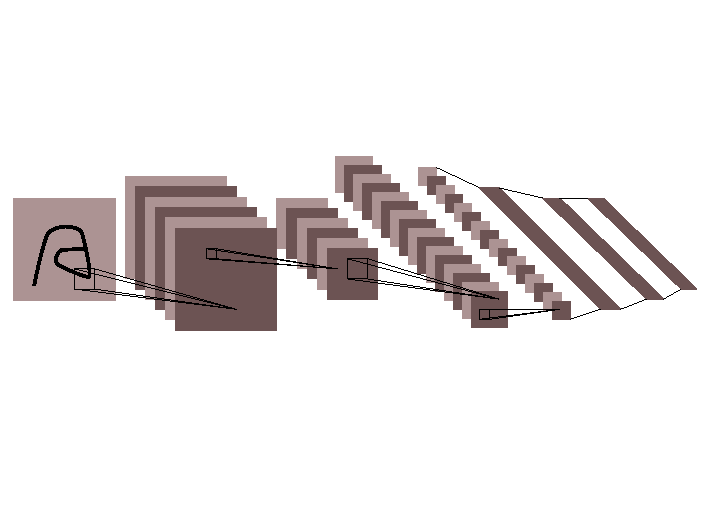
\includegraphics{./pics/lenet.pdf}
\end{frame}

\begin{frame}{Inkscape}
Seminar-related Features:
\begin{enumerate}
    \item Sophisticated painting tool
    \item Cross platform
    \item PSTricks export integrated 
    \item TikZ export available (\href{http://www.inkscapeforum.com/viewtopic.php?t=17898}{Installation})
    \item Beamer drawing template provided
    \item Svg2TikZ
\end{enumerate}
*Other choices: tikzedt, tikzit, latexdraw
\end{frame}

\end{document}
